
\begin{frame}{Глава 3. Движение 1}
    \vspace{-50pt}
    \begin{figure}[h]
        \begin{center}\begin{equation*}\begin{array}{cc}
            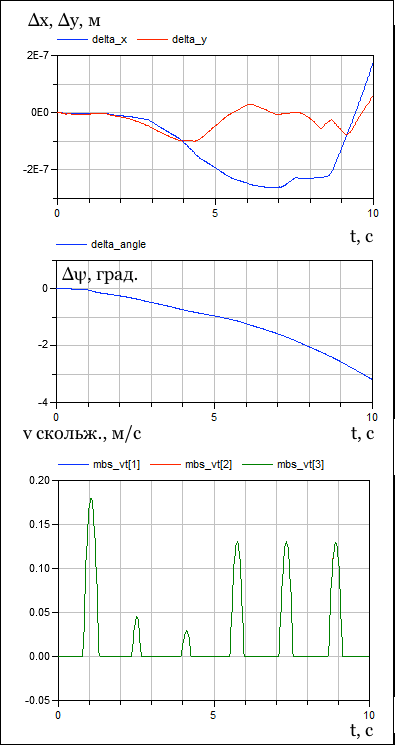
\includegraphics[width=0.4\textwidth, 
            % viewport=0 0 395 745,
            trim=10 20 10 450,
            clip]{content/parts/3_friction/diploma/img/res/comparison_v_0_0_omega_1_frac_1e-1_n_4_time_10s.png} 
            &
            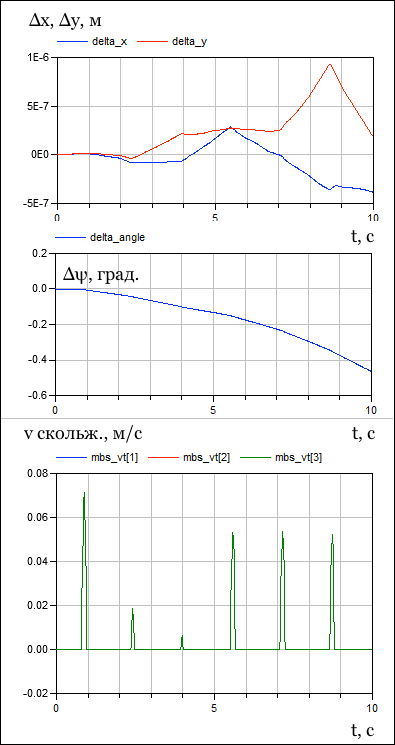
\includegraphics[width=0.4\textwidth, 
            % viewport=0 0 395 745,
            trim=10 20 10 450,
            clip]{content/parts/3_friction/diploma/img/res/comparison_v_0_0_omega_1_frac_1e-2_n_4_time_10s.png}\\
            \ddfrac{m_{\text{рол}}}{m_{\text{к}}} = 10^{-1}, v_0 = 0, \omega_0 = 1 & \ddfrac{m_{\text{рол}}}{m_{\text{к}}} = 10^{-2}, v_0 = 0, \omega_0 = 1\\
        \end{array}\end{equation*}\end{center}
        \caption{Абсолютные величины скоростей скольжения}
    \end{figure}
\end{frame}

\begin{frame}{Глава 3. Движение 1}
    \vspace{-50pt}
    \begin{figure}[h]
        \begin{center}\begin{equation*}\begin{array}{cc}
            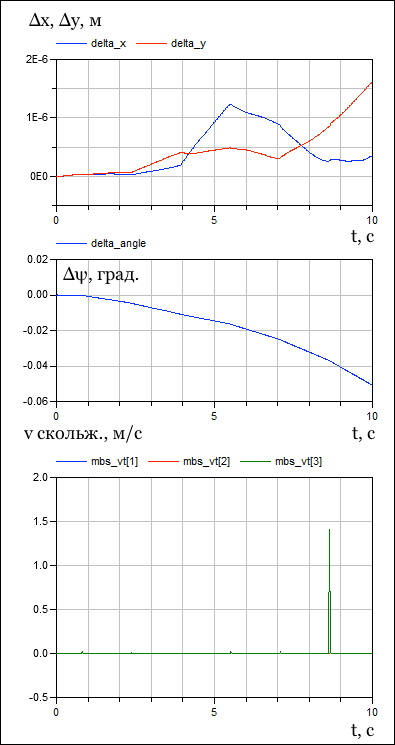
\includegraphics[width=0.4\textwidth,
            % viewport=0 0 395 745,
            trim=10 20 10 450,
            clip]{content/parts/3_friction/diploma/img/res/comparison_v_0_0_omega_1_frac_1e-3_n_4_time_10s.png} 
            &
            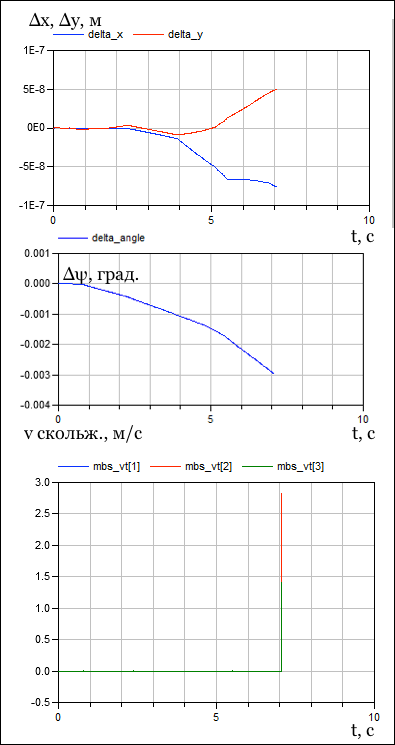
\includegraphics[width=0.4\textwidth, 
            % viewport=0 0 395 745,
            trim=10 20 10 450,
            clip]{content/parts/3_friction/diploma/img/res/comparison_v_0_0_omega_1_frac_1e-4_n_4_time_10s.png}\\
            \ddfrac{m_{\text{рол}}}{m_{\text{к}}} = 10^{-3}, v_0 = 0, \omega_0 = 1 & \ddfrac{m_{\text{рол}}}{m_{\text{к}}} = 10^{-4}, v_0 = 0, \omega_0 = 1\\
        \end{array}\end{equation*}\end{center}
        \caption{Абсолютные величины скоростей скольжения}
    \end{figure}
\end{frame}

\begin{frame}{Глава 3. Движение 1}
    \vspace{-50pt}
    \begin{figure}[h]
        \begin{center}\begin{equation*}\begin{array}{cc}
            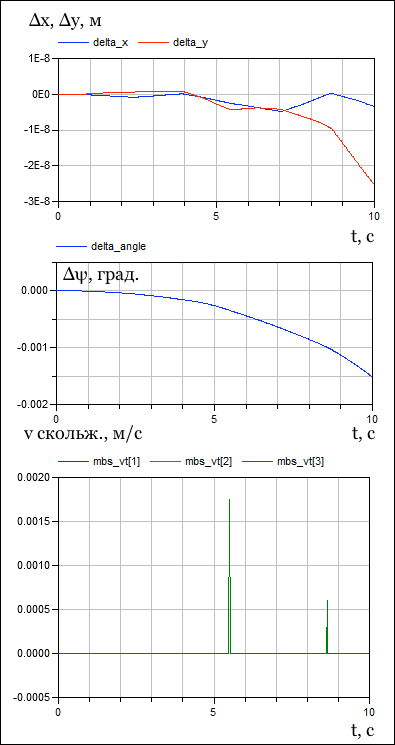
\includegraphics[width=0.4\textwidth, 
            % viewport=0 0 395 745,
            trim=10 20 10 450,
            clip]{content/parts/3_friction/diploma/img/res/comparison_v_0_0_omega_1_frac_1e-5_n_4_time_10s.png} 
            &
            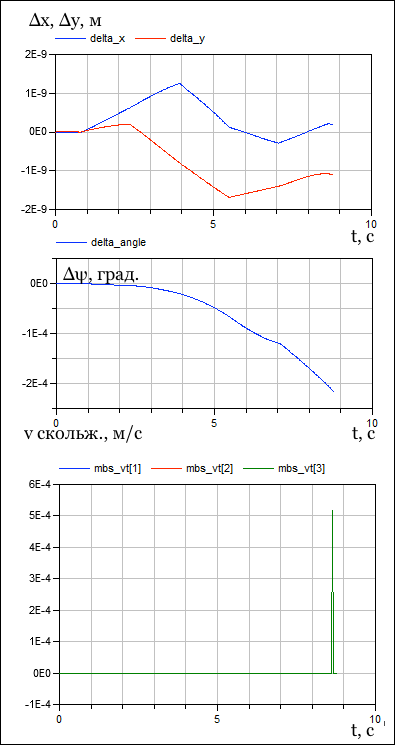
\includegraphics[width=0.4\textwidth, 
            % viewport=0 0 395 745,
            trim=10 20 10 450,
            clip]{content/parts/3_friction/diploma/img/res/comparison_v_0_0_omega_1_frac_1e-6_n_4_time_10s.png}\\
            \ddfrac{m_{\text{рол}}}{m_{\text{к}}} = 10^{-5}, v_0 = 0, \omega_0 = 1 & \ddfrac{m_{\text{рол}}}{m_{\text{к}}} = 10^{-6}, v_0 = 0, \omega_0 = 1\\
        \end{array}\end{equation*}\end{center}
        \caption{Абсолютные величины скоростей скольжения}
    \end{figure}
\end{frame}

\begin{frame}{Глава 3. Движение 2}
    \vspace{-50pt}
    \begin{figure}[h]
        \begin{center}\begin{equation*}\begin{array}{cc}
            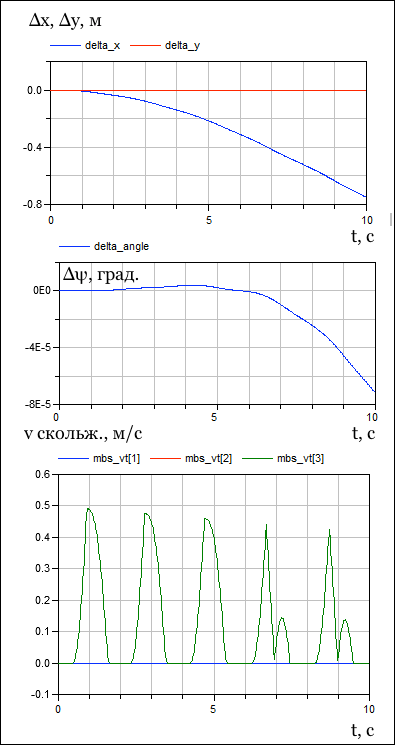
\includegraphics[width=0.4\textwidth, 
            % viewport=0 0 395 745,
            trim=10 20 10 450,
            clip]{content/parts/3_friction/diploma/img/res/comparison_v_1_0_omega_0_frac_1e-1_n_4_time_10s.png}
            &
            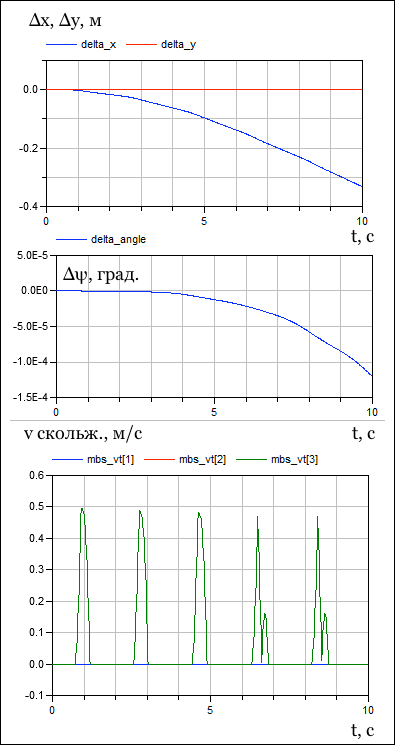
\includegraphics[width=0.4\textwidth, 
            % viewport=0 0 395 745,
            trim=10 20 10 450,
            clip]{content/parts/3_friction/diploma/img/res/comparison_v_1_0_omega_0_frac_1e-2_n_4_time_10s.png}\\
            \ddfrac{m_{\text{рол}}}{m_{\text{к}}} = 10^{-1}, v_0 = 1, \omega_0 = 0 & \ddfrac{m_{\text{рол}}}{m_{\text{к}}} = 10^{-2}, v_0 = 1, \omega_0 = 0\\
        \end{array}\end{equation*}\end{center}
        \caption{Абсолютные величины скоростей скольжения}
    \end{figure}
\end{frame}

\begin{frame}{Глава 3. Движение 2}
    \vspace{-50pt}
    \begin{figure}[h]
        \begin{center}\begin{equation*}\begin{array}{cc}
            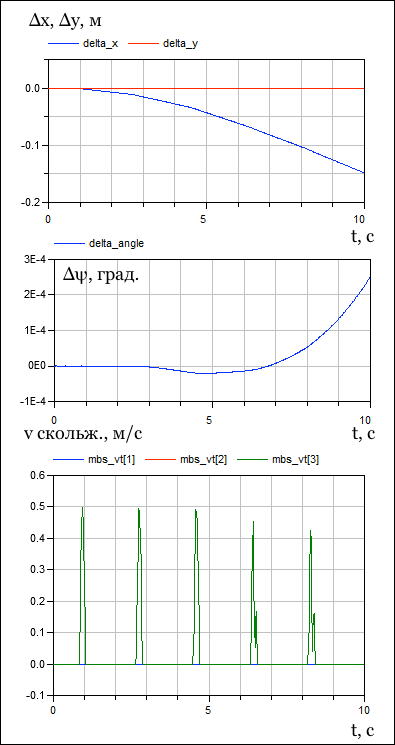
\includegraphics[width=0.4\textwidth,
            % viewport=0 0 395 745,
            trim=10 20 10 450,
            clip]{content/parts/3_friction/diploma/img/res/comparison_v_1_0_omega_0_frac_1e-3_n_4_time_10s.png}
            &
            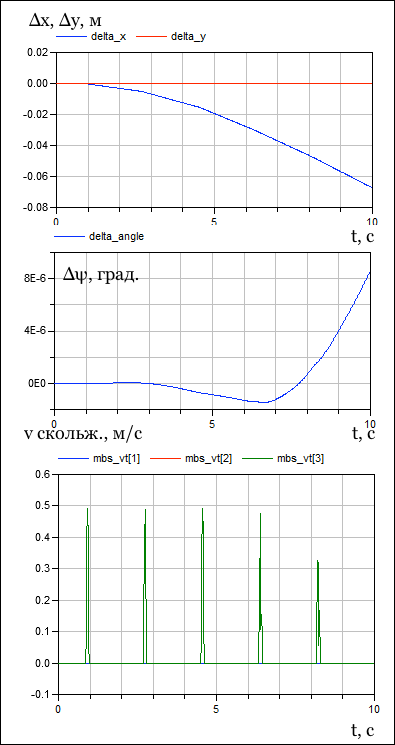
\includegraphics[width=0.4\textwidth, 
            % viewport=0 0 395 745,
            trim=10 20 10 450,
            clip]{content/parts/3_friction/diploma/img/res/comparison_v_1_0_omega_0_frac_1e-4_n_4_time_10s.png}\\
            \ddfrac{m_{\text{рол}}}{m_{\text{к}}} = 10^{-3}, v_0 = 1, \omega_0 = 0 & \ddfrac{m_{\text{рол}}}{m_{\text{к}}} = 10^{-4}, v_0 = 1, \omega_0 = 0\\
        \end{array}\end{equation*}\end{center}
        \caption{Абсолютные величины скоростей скольжения}
    \end{figure}
\end{frame}
